% Template for Cogsci submission with R Markdown

% Stuff changed from original Markdown PLOS Template
\documentclass[10pt, letterpaper]{article}

\usepackage{cogsci}
\usepackage{pslatex}
\usepackage{float}
\usepackage{caption}

% amsmath package, useful for mathematical formulas
\usepackage{amsmath}

% amssymb package, useful for mathematical symbols
\usepackage{amssymb}

% hyperref package, useful for hyperlinks
\usepackage{hyperref}

% graphicx package, useful for including eps and pdf graphics
% include graphics with the command \includegraphics
\usepackage{graphicx}

% Sweave(-like)
\usepackage{fancyvrb}
\DefineVerbatimEnvironment{Sinput}{Verbatim}{fontshape=sl}
\DefineVerbatimEnvironment{Soutput}{Verbatim}{}
\DefineVerbatimEnvironment{Scode}{Verbatim}{fontshape=sl}
\newenvironment{Schunk}{}{}
\DefineVerbatimEnvironment{Code}{Verbatim}{}
\DefineVerbatimEnvironment{CodeInput}{Verbatim}{fontshape=sl}
\DefineVerbatimEnvironment{CodeOutput}{Verbatim}{}
\newenvironment{CodeChunk}{}{}

% cite package, to clean up citations in the main text. Do not remove.
\usepackage{apacite}

% KM added 1/4/18 to allow control of blind submission


\usepackage{color}

% Use doublespacing - comment out for single spacing
%\usepackage{setspace}
%\doublespacing


% % Text layout
% \topmargin 0.0cm
% \oddsidemargin 0.5cm
% \evensidemargin 0.5cm
% \textwidth 16cm
% \textheight 21cm

\title{Using contrast to learn about the world: Listeners' sensitive use of
description to disambiguate referents}


\author{{\large \bf Anonymous}}

\begin{document}

\maketitle

\begin{abstract}
Human listeners are often faced with referential ambiguity. One way they
reduce ambiguity is by using description to narrow down referents.
Beyond narrowing referents to those that match a descriptor, listeners
may infer that a described referent is also one that would have needed
description to be identified uniquely---that it contrasts with other
relevant objects of the same type. This kind of contrastive inference is
known to operate in online processing as listeners try to pick a
referent as a referential utterance progresses (Sedivy et al., 1999;
Sedivy, 2003). However, it is not known whether listeners use this type
of inference to explicitly resolve referential ambiguity: to guide their
choice of a referent. In three experiments, we test whether adult
listeners use color and size adjectives contrastively to guide their
mapping of a novel word onto a novel referent. We find that while they
use size adjectives contrastively to guide referent choice, they do not
do so with color adjectives (Experiment 1). Further, even when color is
described with more relative language (Experiment 2) or emphasized with
prosodic contrastive stress (Experiment 3), participants do not
consistently interpret color contrastively to guide referent choice.

\textbf{Keywords:}
reference resolution; pragmatics; prenominal adjectives
\end{abstract}

\section{Introduction}\label{introduction}

When trying to communicate, human listeners are faced with uncertainty.
Novice listeners---children---face a continuous speech stream filled
with unknown words referring to unformed concepts. Even seasoned
listeners---adults---contend with noise, variable pronunciation,
ambiguous meanings, and the occasional unknown word, too. Fortunately,
listeners bring sensitive phonetic, syntactic, and semantic skills to
the task, allowing them to reduce ambiguity during conversations and
over developmental time (CITE STUFF). Most of these well-documented
skills are concerned with the listener's understanding of the speaker's
utterance alone. But communication occurs in context: in a rich world to
which language refers. Listeners' ability to combine utterance
information with context---their pragmatic ability---may be a powerful
tool in resolving referential ambiguity.

One potential pragmatic tool for reducing referential uncertainty is
contrastive inference. Contrastive inferences are those inferences that
derive from the principle that description should discriminate. This
principle falls out of the more general Gricean maxim that speakers
should say as much as they need to say and no more (Grice, 1975). Given
that communicators strive to be minimal and informative, adjectival
description should discriminate between the referent and some relevant
contrasting set. Sedivy and colleagues performed a visual world task
that demonstrates that adults assume referential description is
contrastive (Sedivy, K. Tanenhaus, Chambers, \& Carlson, 1999). In their
task, four objects appeared on a screen: a target (e.g., a blue cup), a
contrastive pair (e.g., a red cup), a competitor that shares the
target's feature but not category (e.g., a blue comb), and an irrelevant
distractor. Participants then heard a referential expression: ``Pick up
the blue cup.'' Adults looked more quickly to the correct object when
the utterance referred to an object with a same-category contrastive
pair (blue cup vs.~red cup) than when it referred to an object without a
contrastive pair (e.g., the blue comb). Their results suggest that
listeners expect speakers to use description when they are
distinguishing between potential referents of the same type, and
listeners use this inference to rapidly allocate their attention to the
target as an utterance progresses. More recently, this effect was
replicated in 5-year-olds using size adjectives (Huang \& Snedeker,
2008). These experiments demonstrate that listeners interpret at least
some adjectives contrastively, and use this contrastive inference to
guide their attention allocation. These results leave open, however,
whether listeners use contrastive inference to resolve referential
ambiguity and explicitly guide their referent choice.

If listeners are able to use contrastive inference to disambiguate
referents, they may not treat all types of description in the same way.
We may expect the amount of contrastive weight a listener lends an
adjective to vary with its production norms: adjectives that are used
sparingly and contrastively should hold more contrastive weight, while
those that are often used superfluously should hold less. Indeed, there
exist systematic differences in production norms across adjective types.
In English and Dutch, adult speakers are likely to use color adjectives
redundantly, but not size (Mangold \& Pobel, 1988; Pechmann, 1989). Even
5- and 6-year-old English speakers tend to redundantly produce color
adjectives while only producing scalar adjectives to resolve ambiguity
(Nadig \& Sedivy, 2002).

In order to determine whether adults can use contrastive inferences to
disambiguate referents, and how those inferences are affected by
adjective type, we use a reference game with novel objects. Novel
objects provide both a useful experimental tool and an especially
interesting testing ground for contrastive inferences. These objects
avoid effects of typicality and familiarity that relate to level of
description in production (Pechmann, 1989; Rubio-Fernández, 2016) on
particular features (Mangold \& Pobel, 1988). They have unknown names
and feature distributions, creating the ambiguity that is necessary for
our test of referential disambiguation. But the ability to disambiguate
novel referents, or to establish reference with incomplete information,
is also the broader problem of learning about the world. This skill
would aid not only adult speakers dealing with ambiguous or degraded
communicative signal, but also children who need to establish new
word--referent mappings. Across the developmental span, contrastive
inference could help listeners exploit regularities in language and
their environment to learn about both.

\section{Experiment 1}\label{experiment-1}

In Experiment 1, we test whether adult participants use adjective
contrast to choose a novel referent. To examine whether contrast occurs
across adjective types, we test participants in two conditions: color
contrast and size contrast. In a task similar to that of Sedivy and
colleagues (1999), we present participants with arrays of novel fruit
objects. On critical trials, participants see a target object, a lure
object that shares the target's contrast feature but not its shape, and
a contrastive pair that shares the target's shape but not its contrast
feature. Participants hear an utterance denoting the feature: ``Find the
{[}blue/big{]} dax.'' For the target object, use of the adjective is
necessary to disambiguate from the same-shape distractor; for the lure,
the adjective would be superfluous description. If participants use
contrastive inference to choose novel referents, they should choose the
target object. However, we do not expect listeners to treat color and
size equally. Because color is often used redundantly in English while
size is not, we expect size to hold more contrastive weight, encouraging
a more consistent contrastive inference.

\begin{CodeChunk}
\begin{figure}[H]

{\centering 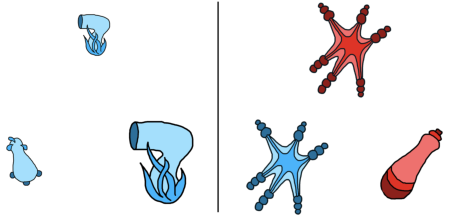
\includegraphics{figs/colortrial-1} 

}

\caption[Example of a contrastive trial in which the critical feature is color]{Example of a contrastive trial in which the critical feature is color. Here, the participant would hear the instruction ``Find the red dax.'' The target is the top object.}\label{fig:colortrial}
\end{figure}
\end{CodeChunk}\begin{CodeChunk}
\begin{figure}[H]

{\centering 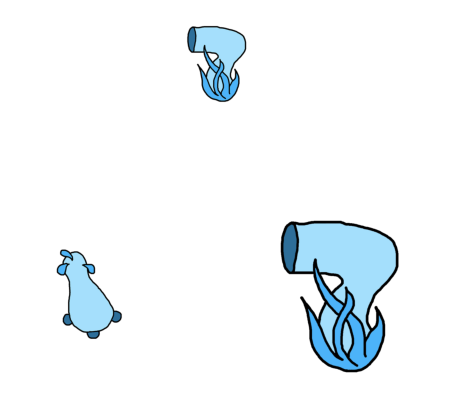
\includegraphics{figs/sizetrial-1} 

}

\caption[Example of a contrastive trial in which the critical feature is size]{Example of a contrastive trial in which the critical feature is size. Here, the participant would hear the instruction ``Find the small dax.'' The target is the top object.}\label{fig:sizetrial}
\end{figure}
\end{CodeChunk}

\subsection{Method}\label{method}

\subsubsection{Participants.}\label{participants.}

100 participants were recruited from Amazon Mechanical Turk. First, 0
were recruited to pilot the task with scalar adjectives. After the
pilot, a full run of the experiment was conducted: 40 participants were
assigned to a condition in which the critical feature was color (stimuli
contrasted on color), and 40 participants were assigned to a condition
in which the critical feature was size.

\subsubsection{Stimuli.}\label{stimuli.}

Stimulus displays were arrays of three novel fruit objects. Fruits were
chosen randomly at each trial from 25 fruit kinds. Ten of the 25 fruit
drawings were adapted and redrawn from {[}citation needed here{]}; we
designed the remaining 15 fruit kinds. Each fruit kind has an instance
in each of four colors (red, blue, green, or purple) and two sizes (big
or small). There were two display types: unique target displays and
contrastive displays. Unique target displays contain a target object
that has a unique shape and is unique on the trial's critical feature
(color or size), and two distractor objects that match each other's (but
not the target's) shape and critical feature. Contrastive displays
contain a target, its contrastive pair (matches the target's shape but
not critical feature), and a lure (matches the target's critical feature
but not shape). The positions of the target and distractor items were
randomized within a triad configuration.

\begin{CodeChunk}
\begin{figure*}[tb]

{\centering 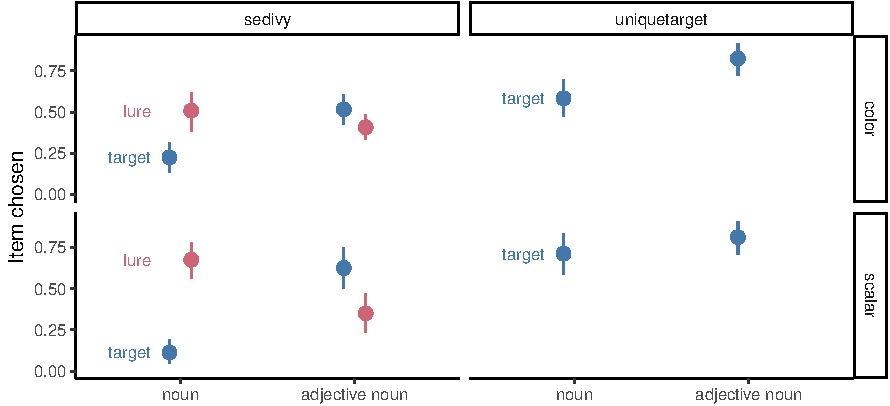
\includegraphics{figs/e1_fig-1} 

}

\caption[Proportion of times that participants chose the target and lure items as a functinon of condition and whether an adjective was provided]{Proportion of times that participants chose the target and lure items as a functinon of condition and whether an adjective was provided. Points indicate group means, error bars indicate 95\% confidence intervals computer by non-parametric bootstrapping}\label{fig:e1_fig}
\end{figure*}
\end{CodeChunk}

\subsubsection{Design and Procedure.}\label{design-and-procedure.}

Participants were told they would play a game in which they would search
for strange alien fruits. In the size condition, each participant saw
eight trials; in the color condition, each participant saw twelve
trials. Half of the trials were unique target displays and half were
contrastive displays. Crossed with display type, half of trials had
audio instructions that described the critical feature of the target
(``Find the {[}blue/big{]} dax''), and half of trials had audio
instructions with no adjective description (``Find the dax''). A name
was randomly chosen at each trial from a list of twelve nonce names:
dax, blicket, wug, toma, gade, sprock, koba, zorp, flib, boti, quen, and
lomet. In the size condition, the size of the target (big or small) was
also crossed with display type and instruction type. All experiment code
is available on GitHub and will be accessible at time of acceptance.

\subsection{Results}\label{results}

We first confirmed that participants understood the task by analyzing
performance on trials in which there was a target unique on both shape
and the relevant contrast adjective. The below results hold for the
pilot with scalar adjectives, but we report values from the full run of
both conditions. We asked whether participants chose the target more
often than expected by chance (\(33\%\)) by fitting a mixed effects
logistic regression with an intercept term, and a random effect of
subject, and an offset of \(logit(1/3)\) to set chance probability to
the correct level. The intercept term was reliably different from zero
for both color (\(\beta =\) 1.13, \(t =\) 4.01, \(p\) \textless{} .001)
and size (\(\beta =\) 7.61, \(t =\) 3.95, \(p\) \textless{} .001). In
addition, participants were more likely to select the target when an
adjective was provided in the audio instruction in both conditions. We
confirmed this effect statistically by fitting a mixed effects logistic
regression predicting target selection from condition, adjective use,
and their interaction with random effects of participants. Adjective
type (color vs.~size) was not statistically related to target choice
(\(\beta =\) 0.99, \(t =\) 1.61, \(p =\) .107), but adjective use
increased target choice (\(\beta =\) 1.93, \(t =\) 4.63, \(p\)
\textless{} .001). The two effects did not interact (\(\beta =\) -1.06,
\(t =\) -1.71, \(p =\) .087). Participants had a general tendency to
choose the target in unique target trials, which was amplified if the
audio instruction contained the relevant contrast adjective.

Our key test was whether participants would choose the target object on
contrastive trials in which description was given, reflecting use of a
contrastive inference to choose a novel referent. To do this, we compare
participants' rate of choosing the target to their rate of choosing the
lure, which shares the relevant contrast feature with the target, when
the audio described the contrast feature. Participants chose the target
more than the lure in the size condition (\(\beta =\) 0.85, \(t =\)
1.97, \(p =\) .049), indicating that participants used size adjectives
to choose the referent contrastively. However, participants in the color
condition did not choose the target significantly more often than they
chose the lure (\(\beta =\) 0.24, \(t =\) 1.23, \(p =\) .218). On
contrastive trials in which a descriptor was not given, participants
dispreferred the target, instead choosing the lure object, which matched
the target on the descriptor but had a unique shape; this was true
across color (\(\beta =\) -1.75, \(t =\) -2.02, \(p =\) .043) and size
(\(\beta =\) -7.96, \(t =\) -3.73, \(p =\) \textless{} .001) conditions.
Adjective use therefore increased target choice (\(\beta =\) 1.37,
\(t =\) 4.59, \(p\) \textless{} .001) across contrastive trials.

\section{Experiment 2}\label{experiment-2}

\begin{CodeChunk}
\begin{figure*}[tb]

{\centering 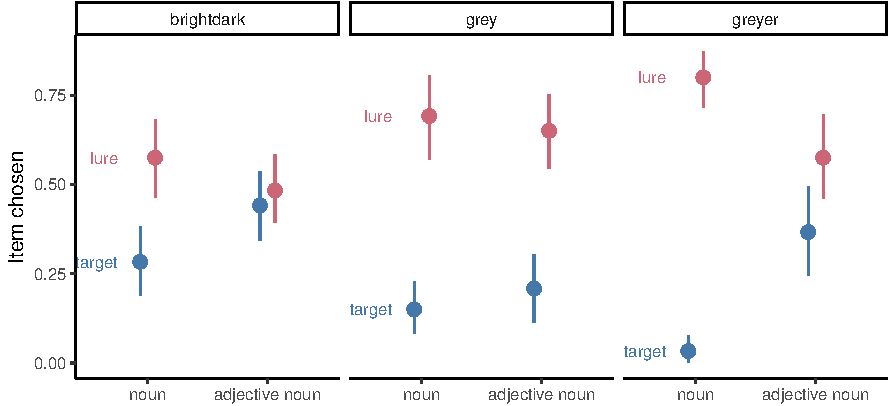
\includegraphics{figs/e2_fig-1} 

}

\caption[Experiment 2]{Experiment 2}\label{fig:e2_fig}
\end{figure*}
\end{CodeChunk}

The results of Experiment 1 demonstrate that adult listeners interpret
color and size adjectives differently, attributing more contrastive
weight to size adjectives and using them to choose novel referents
accordingly. Why might adult listeners do this? As discussed earlier,
participants' responses may reflect a symmetry between adjective
production and comprehension. Since color adjectives are used more
frequently and redundantly than size adjectives, listeners may attenuate
the contrastive weight of color description. A second possibility, not
mutually exclusive with the first, is that size is inherently more
contrastive than color because size is scalar whereas color is more
discrete. Listeners may pay more attention to size contrast because it
occurs on a scale, or interpret it as more contrastive because it is
relative and requires comparison to other category exemplars. In our
second experiment, we aim to examine whether manipulating the
descriptor---making it more or less scalar---of the same stimulus will
change the participants' contrastive inferences about color. To do so,
we present stimuli with varying levels of saturation and value. These
stimuli can be contrasted on either discrete color (blue, grey),
relative color (blueish, greyish), or relative brightness (bright, dark)
adjectives. By maintaining a constant set of stimuli, we rule out
explanations of the contrastive differences between adjective types that
are stimulus-specific---such as some contrasts being more visually
salient---to which our first experiment is susceptible.

\subsection{Methods}\label{methods}

\subsubsection{Participants}\label{participants}

One hundred and twenty participants were recruited from Amazon
Mechanical Turk. Forty participants were assigned to a condition in
which the critical contrast was discrete color (blue, grey), 40
participants were assigned to a condition in which the critical feature
was relative color (blueish, greyish), and 40 participants were assigned
to a condition in which the critical feature was relative brightness
(bright, dark).

\subsubsection{Stimuli}\label{stimuli}

Stimulus displays are arrays of three novel fruit objects, similar to
those used in Experiment 1. Each fruit kind has an instance each of four
colors (red, blue, green, or purple) in two value/saturation levels
(bright and saturated or dark and unsaturated). As in Experiment 1,
there are two display types: unique object displays and contrastive
displays. All fruit objects on any given display are the same hue. In a
unique object display, the target differs from the two distractors in
shape and in value/saturation. In a contrastive display, the target
matches one distractor in shape but not value/saturation, and the other
distractor in value/saturation but not shape (the lure).

\subsubsection{Procedure}\label{procedure}

Instructions and trial structure were identical to Experiment 1.
Displays differed as described above. Audio instructions diverged, this
time reflecting the critical contrasts of each condition: discrete color
(red, blue, green, or purple; or grey), relative color (reddish,
blueish, greenish, or purplish; or greyish), and relative brightness
(bright or dark).

\begin{CodeChunk}
\begin{figure}[H]

{\centering 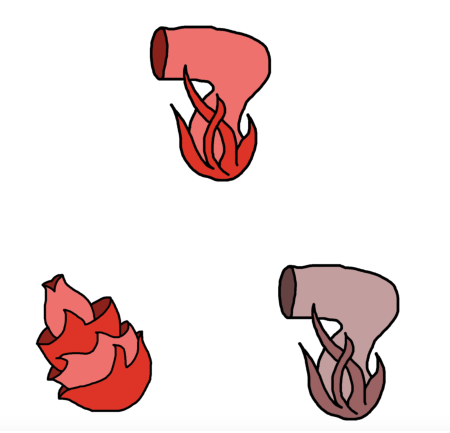
\includegraphics{figs/brightdarktrial-1} 

}

\caption[Example of a contrastive trial in which the critical feature is saturation]{Example of a contrastive trial in which the critical feature is saturation. Here, the participant would hear the instruction ``Find the [red/redder/bright] dax.'' The target is the top object.}\label{fig:brightdarktrial}
\end{figure}
\end{CodeChunk}

\subsection{Results}\label{results-1}

We first analyzed performance on trials in which there was a target
unique on both shape and the relevant contrast adjective, asking whether
participants chose the target more often than expected by chance
(\(33\%\)) by fitting a mixed effects logistic regression with an
intercept term, and a random effect of subject, and an offset of
\(logit(1/3)\) to set chance probability to the correct level. The
intercept term was reliably different from zero for color (e.g., blue,
grey) (\(\beta =\) 4.02, \(t =\) 2.75, \(p\) .006), relative color
(e.g., bluer, greyer) (\(\beta =\) 2.74, \(t =\) 5.31, \(p\) \textless{}
.001), and value (e.g., bright, dark) (\(\beta =\) 2.37, \(t =\) 5.19,
\(p\) \textless{} .001). Adjective type (color vs.~relative color
vs.~bright/dark) was not statistically related to target choice, and
adjective use did not significantly increase target choice (\(\beta =\)
-0.37, \(t =\) -1.05, \(p\) .294).Participants had a general tendency to
choose the target in unique target trials, but there were no significant
main effects of adjective use or adjective type on these trials.

Our key test was whether participants would choose the target object on
contrastive trials when description was given, reflecting use of a
contrastive inference to choose a novel referent. Across all adjective
types, participants did not choose the target significantly more than
they chose the lure, in fact showing a numerical preference for the lure
in each condition and a significant preference for the lure in the
discrete color (e.g., blue, grey) condition (for discrete color:
\(\beta =\) -1.64, \(t =\) -3.34, \(p =\) .001; for relative color:
\(\beta =\) -0.94, \(t =\) -1.84, \(p =\) .066; for value: \(\beta =\)
-0.1, \(t =\) -0.44, \(p =\) .659). Across these conditions,
participants did not consistently demonstrate a contrastive
interpretation in their referent choices, and in fact tended to avoid
contrastive choices.

\section{Experiment 3}\label{experiment-3}

\begin{CodeChunk}
\begin{figure*}[tb]

{\centering 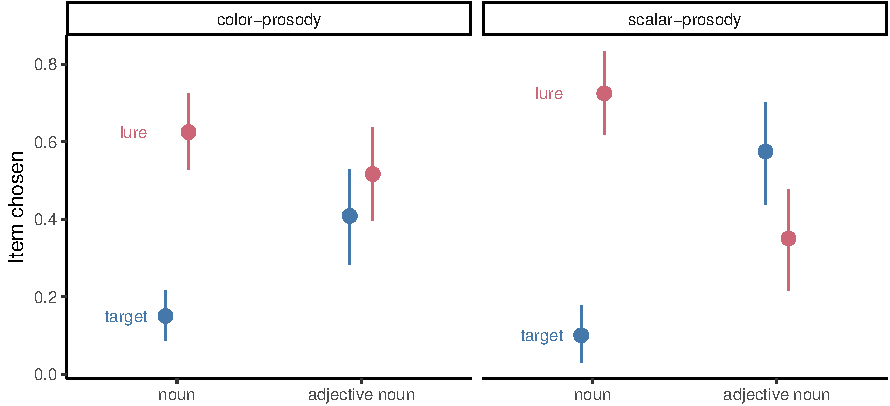
\includegraphics{figs/e3_fig-1} 

}

\caption[Experiment 3]{Experiment 3}\label{fig:e3_fig}
\end{figure*}
\end{CodeChunk}

The results of Experiment 2 suggest that color is not easily interpreted
contrastively, even when descriptors suggest a scalar interpretation.
Given that color has contrastive weight in implicit measures in specific
contexts (Sedivy, 2003; Sedivy et al., 1999), and fails to do so in our
explicit measure, perhaps participants needed a more explicit pragmatic
cue to contrastiveness. To test whether an explicit pragmatic cue would
induce contrastive inferences, in Experiment 3 we manipulate prosody.

The placement of prosodic stress on a word tends to evoke its set of
alternatives, inducing a contrastive interpretation. In early work on
incremental semantic processing (Eberhard, Spivey-Knowlton, Sedivy, \&
Tanenhaus, 1995), participants saw displays containing, for example, a
large blue square, a small blue square, a large yellow circle, and a
small red triangle. Hearing an instruction with contrastive stress on
the size adjective---``Find the \emph{large} blue square''---facilitated
their fixation on the target compared to instructions without
contrastive stress. In Experiment 3, we test whether adding contrastive
stress on the adjective in our instructions facilitates a contrastive
interpretation.

\subsection{Methods}\label{methods-1}

\subsubsection{Participants}\label{participants-1}

Eighty participants were recruited from Amazon Mechanical Turk. Forty
participants were assigned to a condition identical to the color
contrast condition in Experiment 1, with the modification that audio
stimuli included stress on the color adjective. Forty participants were
assigned to a condition identical to the size contrast condition in
Experiment 1, with the modification that audio stimuli included stress
on the size adjective.

\subsubsection{Stimuli}\label{stimuli-1}

Stimulus displays were identical to those in Experiment 1. Audio stimuli
were recorded such that utterances containing an adjective had
contrastive stress on the adjective (e.g., ``Find the \emph{small}
blicket'').

\subsubsection{Procedure}\label{procedure-1}

Instructions and trial structure were identical to Experiment 1.

\subsection{Results}\label{results-2}

We first asked whether participants chose the target more often than
expected by chance (\(33\%\)) on unique target trials by fitting a mixed
effects logistic regression with an intercept term, and a random effect
of subject, and an offset of \(logit(1/3)\) to set chance probability to
the correct level. The intercept term was reliably different from zero
for the color (\(\beta =\) 2.15, \(t =\) 6.25, \(p\) \textless{} .001)
and size (\(\beta =\) 2.58, \(t =\) 4.35, \(p\) \textless{} .001)
conditions. Adjective type (color vs.~size) was not statistically
related to target choice (\(\beta =\) 0.42, \(t =\) 0.77, \(p =\) .444),
but adjective use increased target choice (\(\beta =\) 0.34, \(t =\)
0.92, \(p\) .360).

Our key test was whether participants would choose the target object on
contrastive trials when description was given with contrastive stress,
reflecting use of the descriptor and/or prosodic stress to choose the
referent. In the size condition, participants chose the target more
often than they chose the lure, but this difference did not reach
significance (\(\beta =\) 1.37, \(t =\) 1.44, \(p =\) .151). In the
color condition, participants chose the lure numerically more than they
chose the target, and the difference was not significant (\(\beta =\)
-0.51, \(t =\) -1.09, \(p =\) .277). In this task, contrastive stress
did not seem to encourage a contrastive inference. Though the data
patterned similarly to that of Experiment 1, with participants in the
size condition choosing the target more often than they chose the lure,
this difference did not reach significance.

\section{Discussion}\label{discussion}

In this series of experiments, we asked whether listeners could use
pragmatic contrast to resolve referential ambiguity. Participants were
able to use size adjectives contrastively to establish a novel
word--referent mapping. Their contrastive inference goes beyond the
implicit attention allocation shown in prior eye-tracking paradigms
(Huang \& Snedeker, 2008; Sedivy et al., 1999), determining explicit
referent choice. This finding bolsters contrastive inference as a viable
tool for referential disambiguation.

Participants failed, however, to use color adjectives contrastively in
choosing referents. What makes size different from color? One
possibility is that the scalar nature of size supports a contrastive
interpretation. We tested whether using relative color adjectives (e.g.,
bluer, greyer) or adjectives describing value (bright, dark) on
saturated and desaturated stimuli would encourage the contrastive
inference. We also tested whether adding a prosodic cue to contrast
(e.g., ``Find the \emph{blue} dax'') would encourage contrastive
inference. Participants persisted in interpreting color
non-contrastively, never choosing the intended target significantly
above chance levels. Though we do not claim that contrastive color
inferences cannot be used to explicitly choose referents, it seems that
a contrastive interpretation is difficult to elicit using color, while
it emerges under similar conditions using size.

Another possibility is that color adjectives are often used redundantly,
and therefore receive less contrastive weight than adjectives
consistently used to differentiate between referents. Sedivy puts forth
such an account, finding that adjectives describing material (e.g.,
plastic) and size are interpreted contrastively in eye-tracking
measures, and that this interpretation corresponds to less redundant use
of material and size adjectives in production (Gibson \& Pearlmutter,
2011; Sedivy, 2003). She also finds that color adjectives tend not to be
interpreted contrastively, except in contexts that make their use
unlikely. This account explains well why color is not interpreted
contrastively here, but fails to explain why presumably rare adjectives
(bluer, bright) do not receive contrastive treatment in our task.
Further work is necessary to determine whether contrastive inferences
hew to production norms, and whether implicit indications of contrast
usually extend to explicit referent choice.

Though the participants in our experiments were adults, the ability to
disambiguate novel referents using contrast most obviously serves
budding language learners: children. Contrastive use of adjectives is a
pragmatic regularity in language that children could potentially exploit
to establish word--referent mappings. Tasks using a mixture of novel
adjectives and words suggest that children as young as 3 can make
contrastive inferences about adjectives (Diesendruck, Hall, \& Graham,
2006; Gelman \& Markman, 1985). Five-year-olds demonstrate contrastive
inferences in eye-tracking measures (Huang \& Snedeker, 2008). We plan
to research further the development of these contrastive skills, as well
as their potential as tools for extracting information from language and
context.

\section{Conclusion}\label{conclusion}

We establish here that adult listeners are able to use contrastive
inference to map novel words to novel referents. This ability is
limited, however: it emerges with size but not color description. This
result accords with findings that size adjectives more reliably evoke
contrast in eye-tracking measures (Sedivy, 2003). Our manipulations in
Experiment 2 to make color more relative, which did not result in
contrastive inference, suggest that an explanation of size's effect
based only on its scalar nature is insufficient. An account that relates
production norms to listener interpretation may better explain our
findings. Further research to determine the relationship between
contrastive production and contrastive inference across adjective types,
as well as the relationship between implicit measures of contrastive
inference and explicit referent choice, is ongoing.

\section*{References}\label{references}
\addcontentsline{toc}{section}{References}

\hypertarget{refs}{}
\hypertarget{ref-diesendruck_childrens_2006}{}
Diesendruck, G., Hall, D. G., \& Graham, S. A. (2006). Children's Use of
Syntactic and Pragmatic Knowledge in the Interpretation of Novel
Adjectives. \emph{Child Development}, \emph{77}(1), 16--30.
\url{http://doi.org/10.1111/j.1467-8624.2006.00853.x}

\hypertarget{ref-eberhard_eye_1995}{}
Eberhard, K. M., Spivey-Knowlton, M. J., Sedivy, J. C., \& Tanenhaus, M.
K. (1995). Eye movements as a window into real-time spoken language
comprehension in natural contexts. \emph{Journal of Psycholinguistic
Research}, \emph{24}(6), 409--436.
\url{http://doi.org/10.1007/BF02143160}

\hypertarget{ref-gelman_implicit_1985}{}
Gelman, S. A., \& Markman, E. M. (1985). Implicit contrast in adjectives
vs. nouns: Implications for word-learning in preschoolers*.
\emph{Journal of Child Language}, \emph{12}(1), 125--143.
\url{http://doi.org/10.1017/S0305000900006279}

\hypertarget{ref-gibson_processing_2011}{}
Gibson, E. A., \& Pearlmutter, N. J. (2011). \emph{The Processing and
Acquisition of Reference}. MIT Press.

\hypertarget{ref-grice1975logic}{}
Grice, H. P. (1975). Logic and conversation. \emph{1975}, 41--58.

\hypertarget{ref-huangsnedeker2008}{}
Huang, Y. T., \& Snedeker, J. (2008). Use of referential context in
children's language processing. \emph{Proceedings of the 30th Annual
Meeting of the Cognitive Science Society}.

\hypertarget{ref-mangold_informativeness_1988}{}
Mangold, R., \& Pobel, R. (1988). Informativeness and Instrumentality in
Referential Communication. \emph{Journal of Language and Social
Psychology}, \emph{7}(3-4), 181--191.
\url{http://doi.org/10.1177/0261927X8800700403}

\hypertarget{ref-nadig_evidence_2002}{}
Nadig, A. S., \& Sedivy, J. C. (2002). Evidence of Perspective-Taking
Constraints in Children's On-Line Reference Resolution.
\emph{Psychological Science}, \emph{13}(4), 329--336.
\url{http://doi.org/10.1111/j.0956-7976.2002.00460.x}

\hypertarget{ref-pechmann_incremental_1989}{}
Pechmann, T. (1989). Incremental speech production and referential
overspecification. \emph{Linguistics}, \emph{27}(1), 89--110.
\url{http://doi.org/10.1515/ling.1989.27.1.89}

\hypertarget{ref-rubio-fernandez_how_2016}{}
Rubio-Fernández, P. (2016). How Redundant Are Redundant Color
Adjectives? An Efficiency-Based Analysis of Color Overspecification.
\emph{Frontiers in Psychology}, \emph{7}.
\url{http://doi.org/10.3389/fpsyg.2016.00153}

\hypertarget{ref-sedivy_pragmatic_2003-2}{}
Sedivy, J. C. (2003). Pragmatic Versus Form-Based Accounts of
Referential Contrast: Evidence for Effects of Informativity
Expectations. \emph{Journal of Psycholinguistic Research}, \emph{32}(1),
3--23. \url{http://doi.org/10.1023/A:1021928914454}

\hypertarget{ref-sedivy_achieving_1999}{}
Sedivy, J. C., K. Tanenhaus, M., Chambers, C. G., \& Carlson, G. N.
(1999). Achieving incremental semantic interpretation through contextual
representation. \emph{Cognition}, \emph{71}(2), 109--147.
\url{http://doi.org/10.1016/S0010-0277(99)00025-6}

\bibliographystyle{apacite}


\end{document}
